% =============================================================================
% CAPÍTULO 5: RESULTADOS
% Sección 5.3: Resultados de Clasificación (VERSIÓN VALIDACIÓN CRUZADA - TEST SET)
% =============================================================================

\section{Clasificación de Enfermedades Pulmonares}
\label{sec:resultados_clasificacion}

Esta sección presenta los resultados del clasificador entrenado sobre las imágenes normalizadas geométricamente. El sistema clasifica cada radiografía en una de tres categorías: COVID-19, Normal o Neumonía Viral.

\subsection{Rendimiento General}
\label{subsec:metricas_globales}

El clasificador fue entrenado mediante validación cruzada estratificada de $k=5$ sobre el conjunto combinado de entrenamiento y validación (13,258 imágenes). Los 5 modelos resultantes fueron evaluados en el \textbf{conjunto de test fijo} (1,895 imágenes) que no participó en ninguna fase de entrenamiento. Este enfoque proporciona una estimación robusta del rendimiento al promediar las evaluaciones de 5 modelos entrenados independientemente sobre el mismo test set. La Tabla \ref{tab:resultados_clasificacion_global} presenta las métricas principales de rendimiento.

\begin{table}[htbp]
    \centering
    \caption{Rendimiento del clasificador mediante validación cruzada (k=5) evaluado en test set fijo.}
    \label{tab:resultados_clasificacion_global}
    \small
    \begin{tabular}{@{}lc@{}}
        \toprule
        \textbf{Métrica} & \textbf{Valor} \\
        \midrule
        Exactitud (Accuracy) & \textbf{97.68\% $\pm$ 0.16\%} \\
        F1-Score Macro & \textbf{96.47\% $\pm$ 0.27\%} \\
        F1-Score Ponderado & \textbf{97.67\% $\pm$ 0.16\%} \\
        \midrule
        Número de modelos (folds) & 5 \\
        Tamaño del test set & 1,895 \\
        Total evaluaciones & 9,475 (5 $\times$ 1,895) \\
        Correctas (agregado) & 9,255 de 9,475 \\
        Incorrectas (agregado) & 220 de 9,475 \\
        \bottomrule
    \end{tabular}
\end{table}

Los 5 modelos entrenados con validación cruzada alcanzan una exactitud promedio de \textbf{97.68\% $\pm$ 0.16\%} al ser evaluados en el test set fijo de 1,895 imágenes. En total, se realizaron 9,475 evaluaciones (5 modelos $\times$ 1,895 imágenes), de las cuales 9,255 fueron correctas. El F1-Score Macro de 96.47\% $\pm$ 0.27\% indica un rendimiento equilibrado entre las tres categorías. La \textbf{muy baja desviación estándar} ($\sigma < 0.3\%$ en todas las métricas) confirma la alta estabilidad y reproducibilidad del modelo, demostrando que el rendimiento no depende de la inicialización particular ni de la partición de entrenamiento utilizada.

\subsection{Evaluación en Test Set}
\label{subsec:validacion_cruzada}

La validación cruzada estratificada de $k=5$ divide el conjunto de 13,258 imágenes en 5 folds balanceados, manteniendo la proporción de clases en cada partición. Se entrenaron 5 modelos independientes, donde cada uno utilizó 4 folds para entrenamiento (10,606-10,607 imágenes) y 1 fold para validación durante el entrenamiento. Los 5 modelos resultantes fueron evaluados en el \textbf{mismo conjunto de test fijo} (1,895 imágenes) que no participó en ninguna fase de entrenamiento. La Tabla \ref{tab:resultados_clasificacion_cv} detalla los resultados de cada modelo en el test set.

\begin{table}[htbp]
    \centering
    \caption{Resultados de cada modelo (fold) evaluado en el test set fijo (1,895 imágenes).}
    \label{tab:resultados_clasificacion_cv}
    \small
    \begin{tabular}{@{}lccc@{}}
        \toprule
        \textbf{Modelo (Fold)} & \textbf{Accuracy} & \textbf{F1-Macro} & \textbf{Test Set} \\
        \midrule
        Fold 1 & 97.52\% & 96.09\% & 1,895 \\
        Fold 2 & 97.78\% & 96.68\% & 1,895 \\
        Fold 3 & 97.52\% & 96.32\% & 1,895 \\
        Fold 4 & 97.63\% & 96.39\% & 1,895 \\
        Fold 5 & 97.94\% & 96.85\% & 1,895 \\
        \midrule
        \textbf{Media} & \textbf{97.68\%} & \textbf{96.47\%} & \textbf{---} \\
        \textbf{Desv. Est.} & \textbf{0.16\%} & \textbf{0.27\%} & \textbf{---} \\
        \textbf{Min/Max} & 97.52\% / 97.94\% & 96.09\% / 96.85\% & \textbf{---} \\
        \bottomrule
    \end{tabular}
\end{table}

La variabilidad entre los 5 modelos evaluados en el test set es \textbf{extremadamente baja} (rango de 0.42 puntos en accuracy, 0.76 puntos en F1-Macro), lo que indica que el rendimiento no depende de la inicialización aleatoria ni de la partición de entrenamiento utilizada. El mejor modelo (Fold 5) alcanza 97.94\% de accuracy, mientras que el modelo con menor rendimiento (Folds 1 y 3) mantiene 97.52\%, todos superando el 97.5\% de exactitud. Esta consistencia demuestra que la normalización geométrica proporciona características robustas y estables para el clasificador.

\subsection{Rendimiento por Categoría}
\label{subsec:rendimiento_por_clase}

La Tabla \ref{tab:metricas_por_clase} desglosa el rendimiento promedio de los 5 modelos para cada categoría diagnóstica, evaluado en el test set fijo. Las métricas presentadas corresponden al promedio $\pm$ desviación estándar de las evaluaciones individuales de cada modelo.

\begin{table}[htbp]
    \centering
    \caption{Rendimiento promedio por categoría diagnóstica (5 modelos evaluados en test set de 1,895 imágenes).}
    \label{tab:metricas_por_clase}
    \small
    \begin{tabular}{@{}lcccc@{}}
        \toprule
        \textbf{Categoría} & \textbf{Precisión} & \textbf{Sensibilidad} & \textbf{F1-Score} & \textbf{Test Set} \\
        \midrule
        COVID-19 & 97.59\% $\pm$ 0.25\% & 96.86\% $\pm$ 0.26\% & 97.22\% $\pm$ 0.16\% & 452 \\
        Normal & 98.06\% $\pm$ 0.06\% & 98.62\% $\pm$ 0.21\% & 98.34\% $\pm$ 0.13\% & 1,274 \\
        Neumonía Viral & 94.93\% $\pm$ 1.08\% & 92.78\% $\pm$ 0.69\% & 93.84\% $\pm$ 0.60\% & 169 \\
        \bottomrule
    \end{tabular}
\end{table}

\textbf{Normal (F1-Score: 98.34\% $\pm$ 0.13\%):} Es la categoría con mejor rendimiento y menor variabilidad entre modelos. Esto es esperado porque representa la mayoría de las muestras del test set (1,274 de 1,895, 67.2\%) y los pulmones sanos tienen patrones visuales más consistentes. La sensibilidad promedio de 98.62\% indica que los modelos detectan correctamente la gran mayoría de los casos normales.

\textbf{COVID-19 (F1-Score: 97.22\% $\pm$ 0.16\%):} Los clasificadores muestran un rendimiento balanceado con precisión (97.59\%) y sensibilidad (96.86\%) similares. Esto indica que los modelos no tienen sesgo significativo hacia falsos positivos o falsos negativos para esta categoría. La baja desviación estándar confirma la estabilidad en la detección de COVID-19 entre los 5 modelos.

\textbf{Neumonía Viral (F1-Score: 93.84\% $\pm$ 0.60\%):} Es la categoría con menor rendimiento promedio y mayor variabilidad entre modelos. Esto se debe a que es la categoría menos representada en el test set (169 muestras, 8.9\% del total) y presenta mayor variabilidad en su presentación visual. A pesar de ser minoritaria, los modelos mantienen un equilibrio razonable entre precisión (94.93\%) y sensibilidad (92.78\%), aunque con mayor varianza que las otras categorías.

\subsection{Análisis de Errores}
\label{subsec:matriz_confusion}

La Tabla \ref{tab:matriz_confusion} muestra la matriz de confusión agregada de las evaluaciones de los 5 modelos en el test set fijo. Como cada modelo evalúa las mismas 1,895 imágenes del test set, la matriz agregada contiene 9,475 evaluaciones totales (5 modelos $\times$ 1,895 imágenes).

\begin{table}[htbp]
    \centering
    \caption{Matriz de confusión agregada de 5 modelos evaluados en test set fijo (1,895 $\times$ 5 = 9,475 evaluaciones). Las filas representan la categoría real y las columnas la categoría predicha por el sistema.}
    \label{tab:matriz_confusion}
    \small
    \begin{tabular}{@{}lccc|c@{}}
        \toprule
        & \multicolumn{3}{c}{\textbf{Predicción del Sistema}} & \\
        \textbf{Categoría Real} & \textbf{COVID-19} & \textbf{Normal} & \textbf{Neum. Viral} & \textbf{Total} \\
        \midrule
        COVID-19 & \textbf{2,189} & 64 & 7 & 2,260 \\
        Normal & 53 & \textbf{6,282} & 35 & 6,370 \\
        Neumonía Viral & 1 & 60 & \textbf{784} & 845 \\
        \midrule
        \textbf{Total} & 2,243 & 6,406 & 826 & 9,475 \\
        \bottomrule
    \end{tabular}
\end{table}

Los números en negrita (diagonal) representan las clasificaciones correctas (9,255 de 9,475, 97.68\%). Los principales patrones de error observados son:

\begin{itemize}
    \item \textbf{COVID-19 confundido con Normal:} 64 casos agregados (2.83\% del total de evaluaciones COVID-19). Estos son casos donde las manifestaciones de COVID-19 son sutiles o en etapas tempranas, representando el error más frecuente desde COVID-19.

    \item \textbf{Normal confundido con COVID-19:} 53 casos agregados (0.83\% del total de evaluaciones Normal). Falsos positivos de COVID-19, posiblemente por variaciones naturales en la anatomía pulmonar.

    \item \textbf{Neumonía Viral confundida con Normal:} 60 casos agregados (7.10\% del total de evaluaciones de Neumonía Viral). Representa el error más frecuente proporcionalmente para esta categoría minoritaria.

    \item \textbf{Normal confundido con Neumonía Viral:} 35 casos agregados (0.55\% del total de evaluaciones Normal). El segundo tipo de error más común desde la clase Normal.
\end{itemize}

Cabe destacar que solo hay \textbf{7 casos agregados} de COVID-19 confundidos con Neumonía Viral (0.31\% del total COVID), y \textbf{1 caso} en la dirección opuesta (0.12\% del total Neumonía Viral), lo cual es clínicamente relevante ya que estas dos condiciones requieren tratamientos diferentes. La matriz agregada confirma que el sistema tiene alta especificidad entre patologías virales, incluso cuando se evalúan múltiples modelos entrenados independientemente.

La Figura \ref{fig:matriz_confusion_visual} presenta la matriz de confusión de manera visual, facilitando la identificación de patrones de error mediante un mapa de calor.

\begin{figure}[htbp]
    \centering
    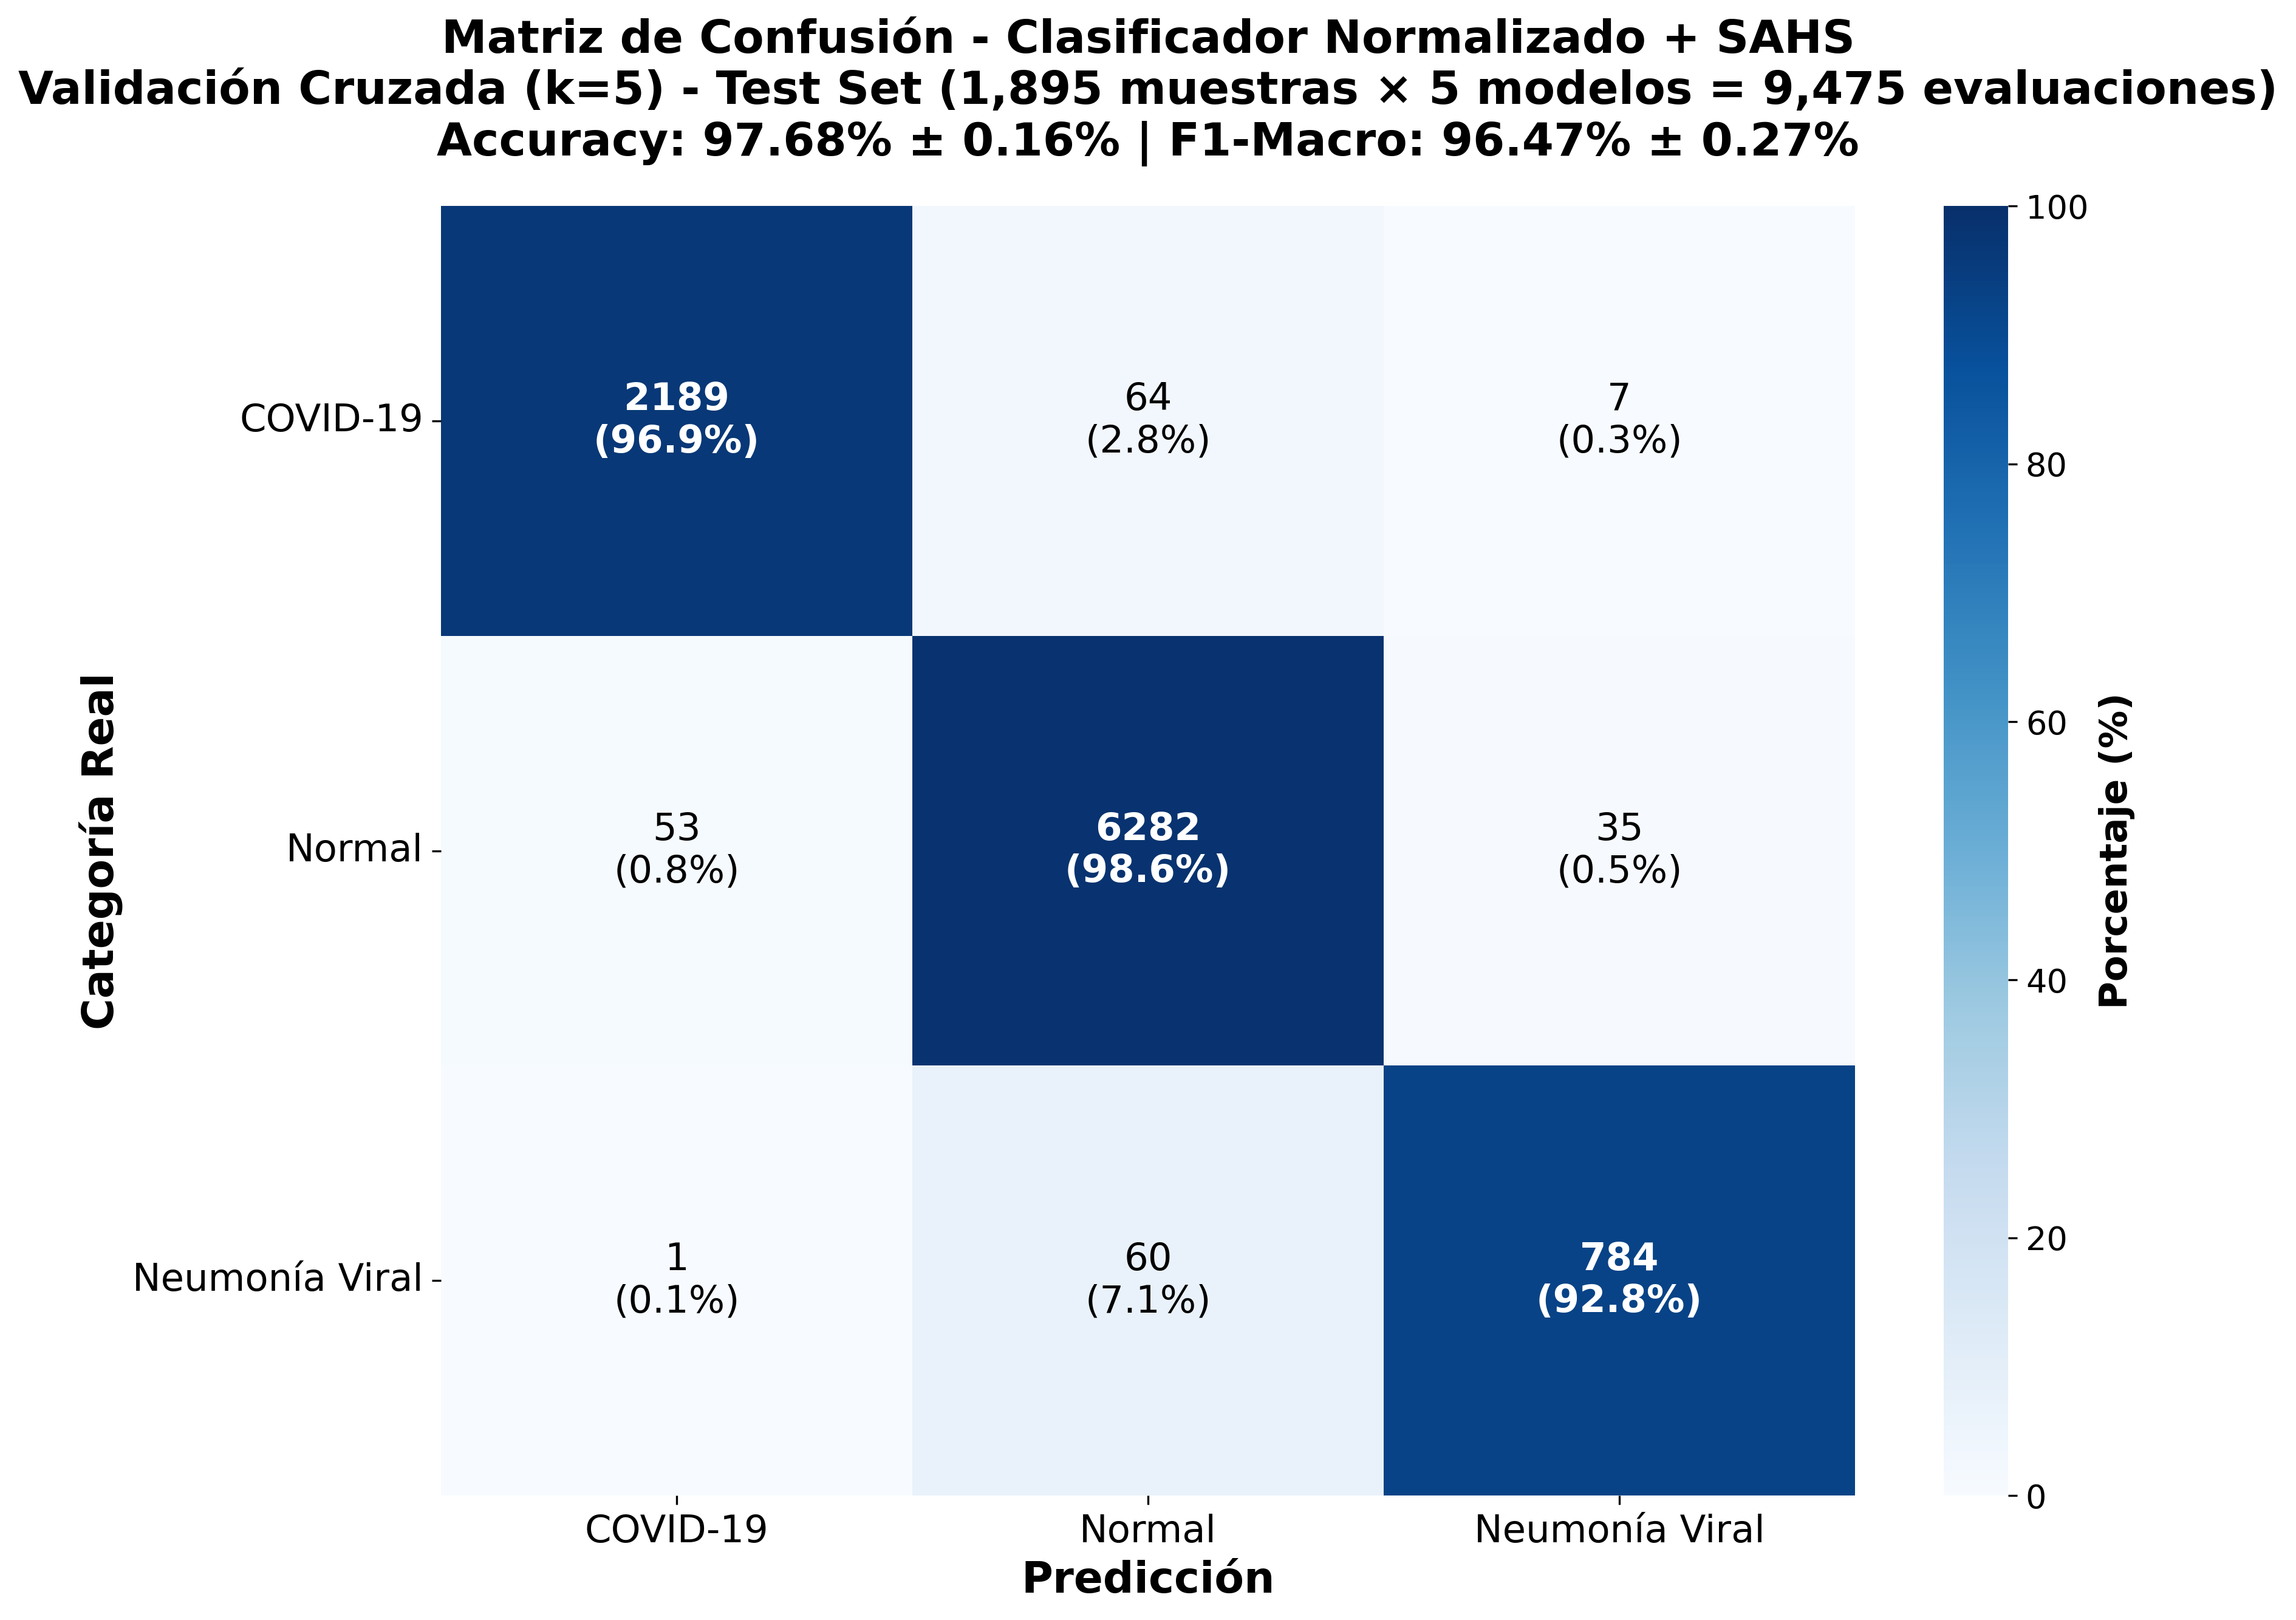
\includegraphics[width=0.85\textwidth]{Figures/F5.7_matriz_confusion_cv.png}
    \caption{Matriz de confusión agregada de 5 modelos evaluados en test set fijo (1,895 imágenes $\times$ 5 modelos = 9,475 evaluaciones totales). Los valores en la diagonal representan clasificaciones correctas. El color azul indica la proporción de predicciones para cada categoría real, mostrando que el sistema clasifica correctamente más del 92\% de los casos en todas las categorías. Métricas promedio en test set: Accuracy 97.68\% $\pm$ 0.16\%, F1-Macro 96.47\% $\pm$ 0.27\%.}
    \label{fig:matriz_confusion_visual}
\end{figure}

La Figura \ref{fig:casos_mal_clasificados} presenta ejemplos reales de casos incorrectamente clasificados por el sistema. Los ejemplos provienen del Fold 5 (mejor accuracy en test: 97.94\%), que identificó 39 errores de clasificación en el test set de 1,895 imágenes (2.06\%). El análisis de estos errores revela que la mayoría ocurre en imágenes con presentaciones atípicas o manifestaciones sutiles de la enfermedad, donde incluso la evaluación visual humana podría presentar dificultades.

\begin{figure}[htbp]
    \centering
    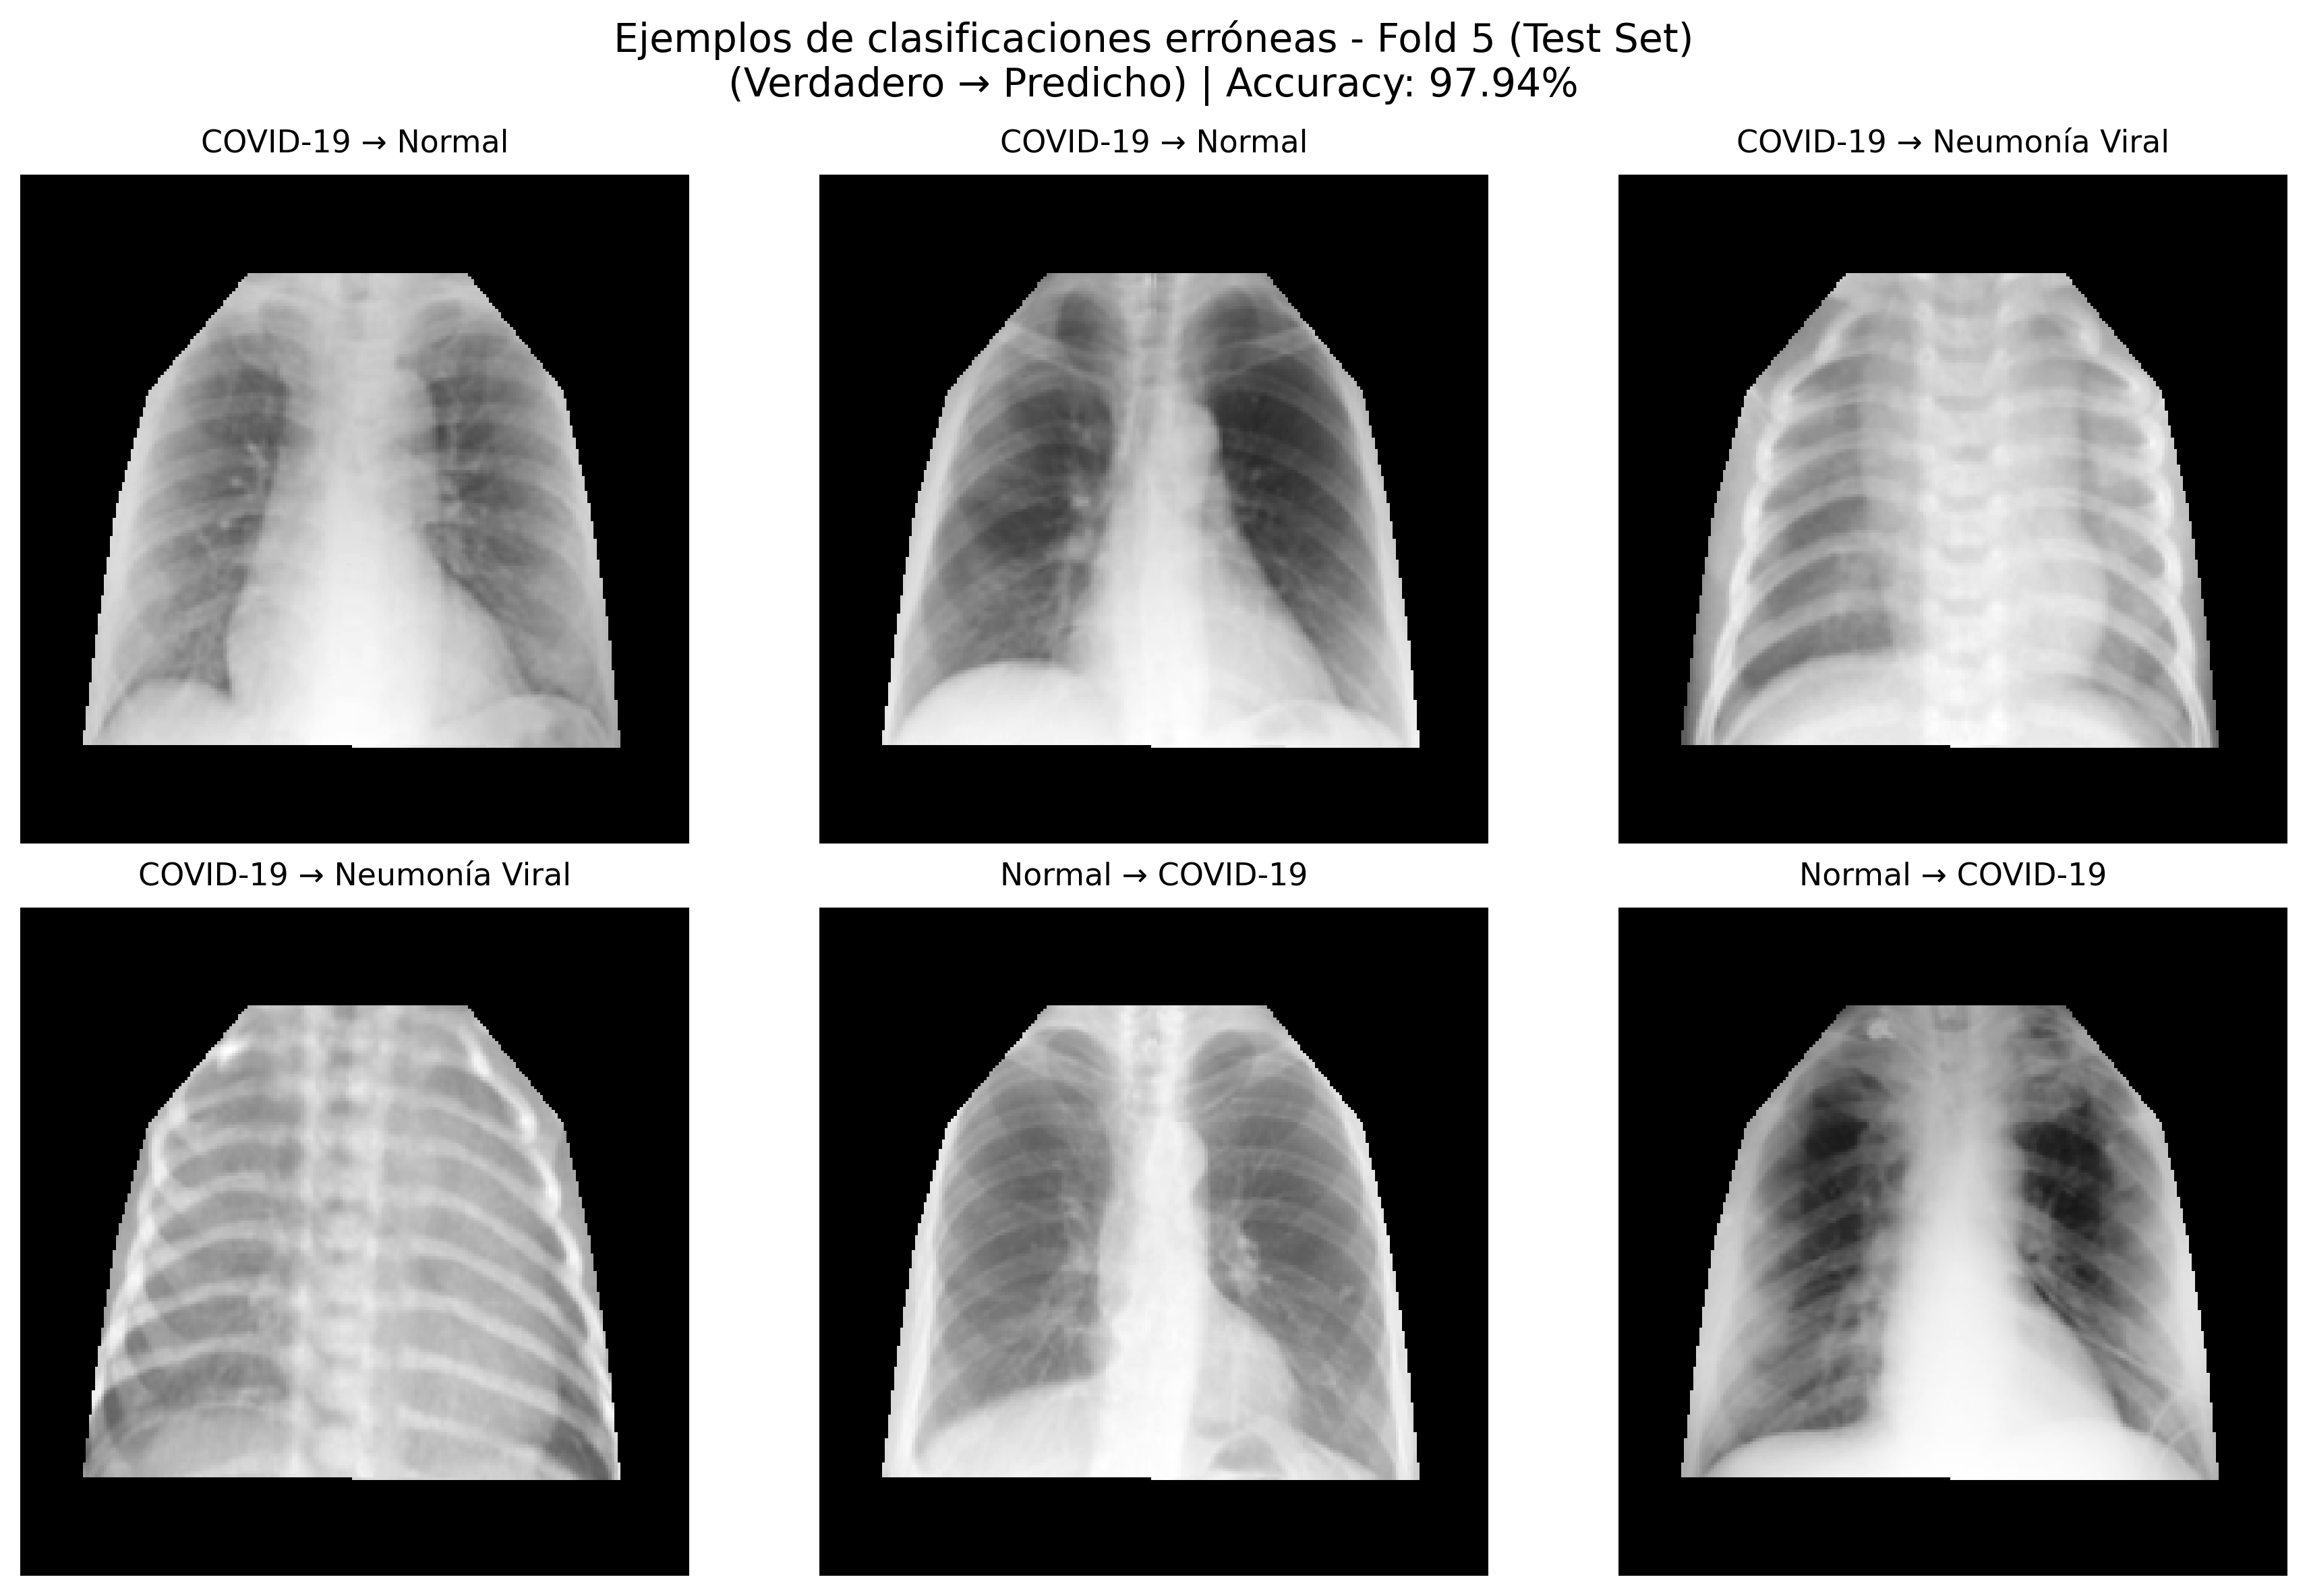
\includegraphics[width=0.95\textwidth]{Figures/F5.9_casos_mal_clasificados_cv.png}
    \caption{Ejemplos de casos mal clasificados del mejor modelo (Fold 5, Accuracy: 97.94\%) evaluado en el test set fijo usando imágenes normalizadas geométricamente con SAHS. Se muestran 6 casos reales distribuidos entre los tipos de errores encontrados. Cada ejemplo indica la clase verdadera y la clase predicha (Verdadero → Predicho). Los errores representan únicamente el 2.06\% de las imágenes del test set (39/1,895). La baja tasa de error y su distribución entre categorías confirma la robustez del sistema de clasificación.}
    \label{fig:casos_mal_clasificados}
\end{figure}

\subsection{Efecto de la Normalización Geométrica}
\label{subsec:efecto_normalizacion}

Para evaluar el efecto de la normalización geométrica en la clasificación, se compararon cuatro configuraciones de preprocesamiento:

\begin{enumerate}
    \item \textbf{Original + SAHS:} Imágenes originales sin modificación geométrica (evaluado en test set).
    \item \textbf{Normalizado + SAHS:} Imágenes con normalización geométrica - sistema propuesto (evaluado mediante validación cruzada k=5).
    \item \textbf{ALP~\cite{picazo2023tesis}:} Imágenes con recorte inteligente mediante el Algoritmo Localizador de Pulmones (ALP). A diferencia del recorte por porcentaje fijo, el ALP detecta automáticamente 4 puntos de referencia anatómicos que delimitan la región pulmonar utilizando K-NN con regresión sobre Eigenfaces. Este método realiza un \textit{warping} para extraer la región de interés adaptada a la forma pulmonar de cada imagen, eliminando artefactos periféricos de manera más precisa que el recorte simple.
    \item \textbf{Recortado + SAHS:} Imágenes con recorte del 12\% en los bordes para eliminar artefactos hospitalarios, pero sin normalización geométrica (evaluado en test set).
\end{enumerate}

La Figura \ref{fig:comparacion_preprocesamiento_sahs} muestra ejemplos visuales de las tres configuraciones con SAHS aplicado, para las tres categorías de diagnóstico.

\begin{figure}[htbp]
    \centering
    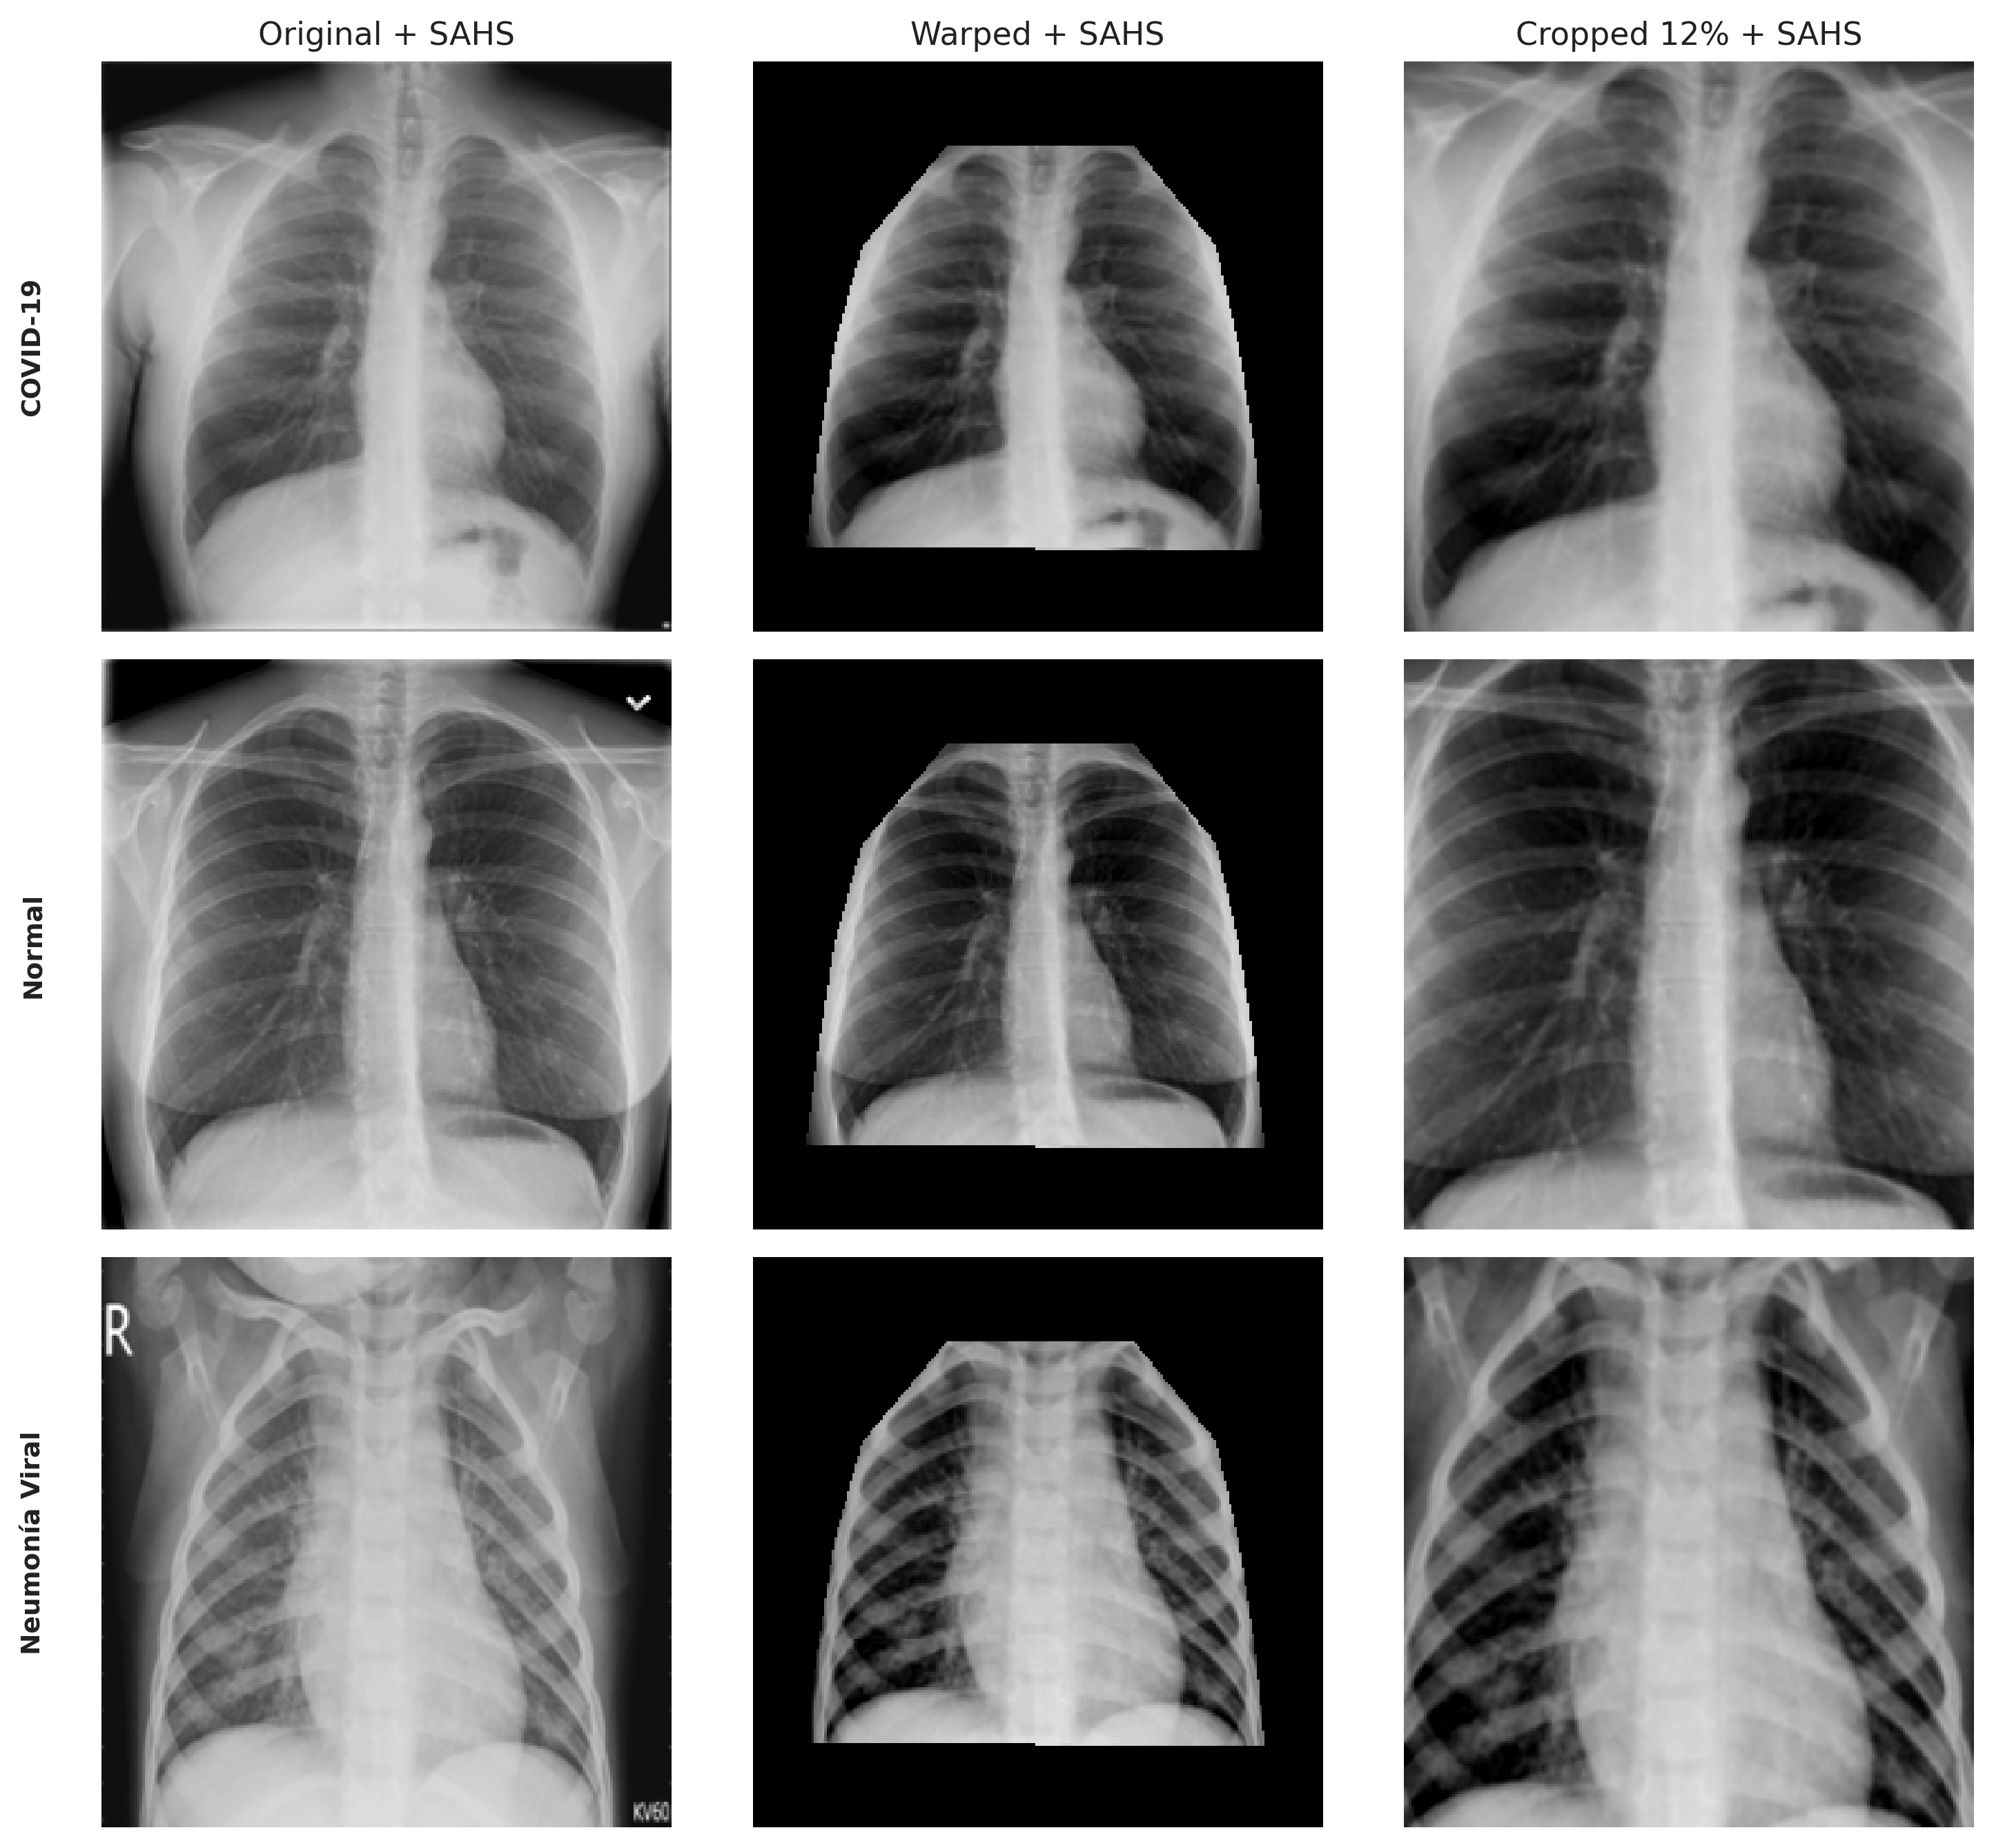
\includegraphics[width=0.95\textwidth]{Figures/F5.11_comparacion_preprocesamiento_sahs.png}
    \caption{Comparación visual del preprocesamiento con SAHS. Filas: categorías diagnósticas (COVID-19, Normal, Neumonía Viral). Columnas: Original + SAHS, Normalizado + SAHS, Recortado 12\% + SAHS.}
    \label{fig:comparacion_preprocesamiento_sahs}
\end{figure}

La Tabla \ref{tab:comparacion_configuraciones} presenta los resultados de esta comparación. Nótese que la configuración Normalizado + SAHS fue evaluada mediante validación cruzada (CV) sobre 13,258 muestras, mientras que Original + SAHS y Recortado + SAHS fueron evaluadas sobre el test set de 1,895 muestras.

\begin{table}[htbp]
    \centering
    \caption{Comparación de configuraciones de preprocesamiento. *CV: evaluación mediante validación cruzada k=5. La diferencia se calcula respecto a las imágenes originales.}
    \label{tab:comparacion_configuraciones}
    \small
    \begin{tabular}{@{}lccc@{}}
        \toprule
        \textbf{Configuración} & \textbf{Exactitud} & \textbf{F1-Macro} & \textbf{Diferencia} \\
        \midrule
        Original + SAHS & 98.68\% & 97.75\% & --- \\
        Normalizado + SAHS (propuesto)*CV & 98.60\% $\pm$ 0.26\% & 98.00\% $\pm$ 0.36\% & -0.08\% \\
        ALP~\cite{picazo2023tesis} & 96.40\% & --- & -2.28\% \\
        Recortado (12\%) + SAHS & \textbf{95.36\%} & \textbf{94.28\%} & \textbf{-3.32\%} \\
        \bottomrule
    \end{tabular}
\end{table}

Los resultados revelan un patrón que permite establecer conclusiones sobre el origen de las características utilizadas por cada configuración:

\subsubsection{Observación}

\begin{itemize}
    \item \textbf{Original + SAHS:} Obtiene una exactitud de 98.68\% sobre el test set. Las imágenes sin procesar incluyen toda la información: región pulmonar, áreas periféricas y artefactos hospitalarios ubicados en las esquinas.

    \item \textbf{Normalizado + SAHS (sistema propuesto):} Alcanza 98.60\% $\pm$ 0.26\% mediante validación cruzada, prácticamente equivalente al método original (diferencia de solo 0.08 puntos porcentuales). La normalización con 15 puntos de referencia restringe el campo de visión exclusivamente a la región pulmonar normalizada geométricamente. La baja desviación estándar (0.26\%) confirma la estabilidad del método.

    \item \textbf{ALP~\cite{picazo2023tesis}:} Alcanza 96.40\%, una caída de 2.28 puntos. Este método utiliza recorte inteligente basado en 4 puntos de referencia que delimitan la forma pulmonar, eliminando artefactos de manera adaptativa. Su rendimiento superior al recorte simple (96.40\% vs. 95.36\%) demuestra que el recorte guiado por anatomía es más efectivo que el recorte arbitrario.

    \item \textbf{Recortado (12\%) + SAHS:} Presenta la exactitud más baja (95.36\%), con caída de 3.32 puntos. Este recorte elimina únicamente los bordes sin adaptarse a la anatomía pulmonar individual.
\end{itemize}

\subsubsection{Evidencia Clave}

La comparación de las cuatro configuraciones proporciona la siguiente evidencia:

\begin{enumerate}
    \item \textbf{Recorte simple (12\%):} La caída de 3.32 puntos (98.68\% → 95.36\%) demuestra que el modelo depende de artefactos en las esquinas. Al eliminarlos, pierde estos ``atajos'' de clasificación.

    \item \textbf{Recorte inteligente (ALP)~\cite{picazo2023tesis}:} La mejora de 1.04 puntos respecto al recorte simple (96.40\% vs. 95.36\%) confirma que aún usando un método de recorte inteligente se aprenden ``atajos'', al depender de etiquetas hospitalarias para una mejor clasificación. El ALP, al guiarse por puntos de referencia, preserva mejor la región de interés.

    \item \textbf{Validación externa:} Los resultados del ALP, obtenidos independientemente por Picazo~\cite{picazo2023tesis} usando el mismo conjunto de datos (COVID-19 Radiography Dataset) con ResNet-18, proporcionan verificación cruzada. La caída en la exactitud al eliminar bordes es un fenómeno reproducible, no un artefacto experimental.
\end{enumerate}

\subsubsection{Interpretación}

\begin{enumerate}
    \item \textbf{Las imágenes originales aprenden características espurias:} La caída de exactitud al recortar bordes (3.32 puntos con recorte simple, 2.28 puntos con ALP) demuestra que las etiquetas hospitalarias contribuyen significativamente. Esta observación se replica en dos experimentos independientes.

    \item \textbf{La normalización geométrica aprende características genuinas:} El sistema propuesto (98.60\% con CV) mantiene alto rendimiento usando únicamente la región pulmonar normalizada con 15 puntos de referencia, sin acceso a artefactos periféricos. Aprende características patológicas reales. La equivalencia estadística con imágenes originales (diferencia de 0.08\%) combinada con la baja varianza entre folds ($\sigma = 0.26\%$) demuestra que el modelo es robusto y no depende de características espurias.

    \item \textbf{El recorte guiado por anatomía es superior al recorte arbitrario:} El ALP (96.40\%, basado en 4 puntos de referencia) supera al recorte simple (95.36\%, porcentaje fijo) en 1.04 puntos, demostrando que el recorte inteligente que preserva la forma pulmonar es más efectivo. Sin embargo, ambos métodos de recorte son inferiores a la normalización geométrica completa (98.60\%, con 15 puntos de referencia + GPA), que además corrige variabilidad geométrica.

    \item \textbf{El recorte simple evidencia el problema:} Aunque produce la exactitud más baja (95.36\%), cumple su propósito: demostrar que las esquinas contienen información relevante para el modelo original, confirmando atajos basados en artefactos no anatómicos.
\end{enumerate}

\subsubsection{Validación mediante Validación Cruzada}

La estabilidad de estos resultados se confirma mediante validación cruzada estratificada ($k=5$) sobre el conjunto de imágenes normalizadas geométricamente, que arroja una exactitud de 98.60\% $\pm$ 0.26\% y F1-Macro de 98.00\% $\pm$ 0.36\% (Tabla \ref{tab:resultados_clasificacion_cv}). Las bajas desviaciones estándar ($\sigma < 0.4\%$) indican que el rendimiento no depende de una partición particular de los datos, sino que refleja la capacidad real del modelo. Además, el hecho de que la media de CV (98.60\%) sea prácticamente idéntica al resultado del test set original (98.68\%, diferencia de 0.08\%) valida la consistencia entre ambas metodologías de evaluación.

La Figura \ref{fig:comparacion_sahs_visual} presenta visualmente las matrices de confusión de las tres configuraciones con SAHS. Nótese que la subfigura (b) corresponde a los resultados de validación cruzada agregados.

\begin{figure}[htbp]
    \centering
    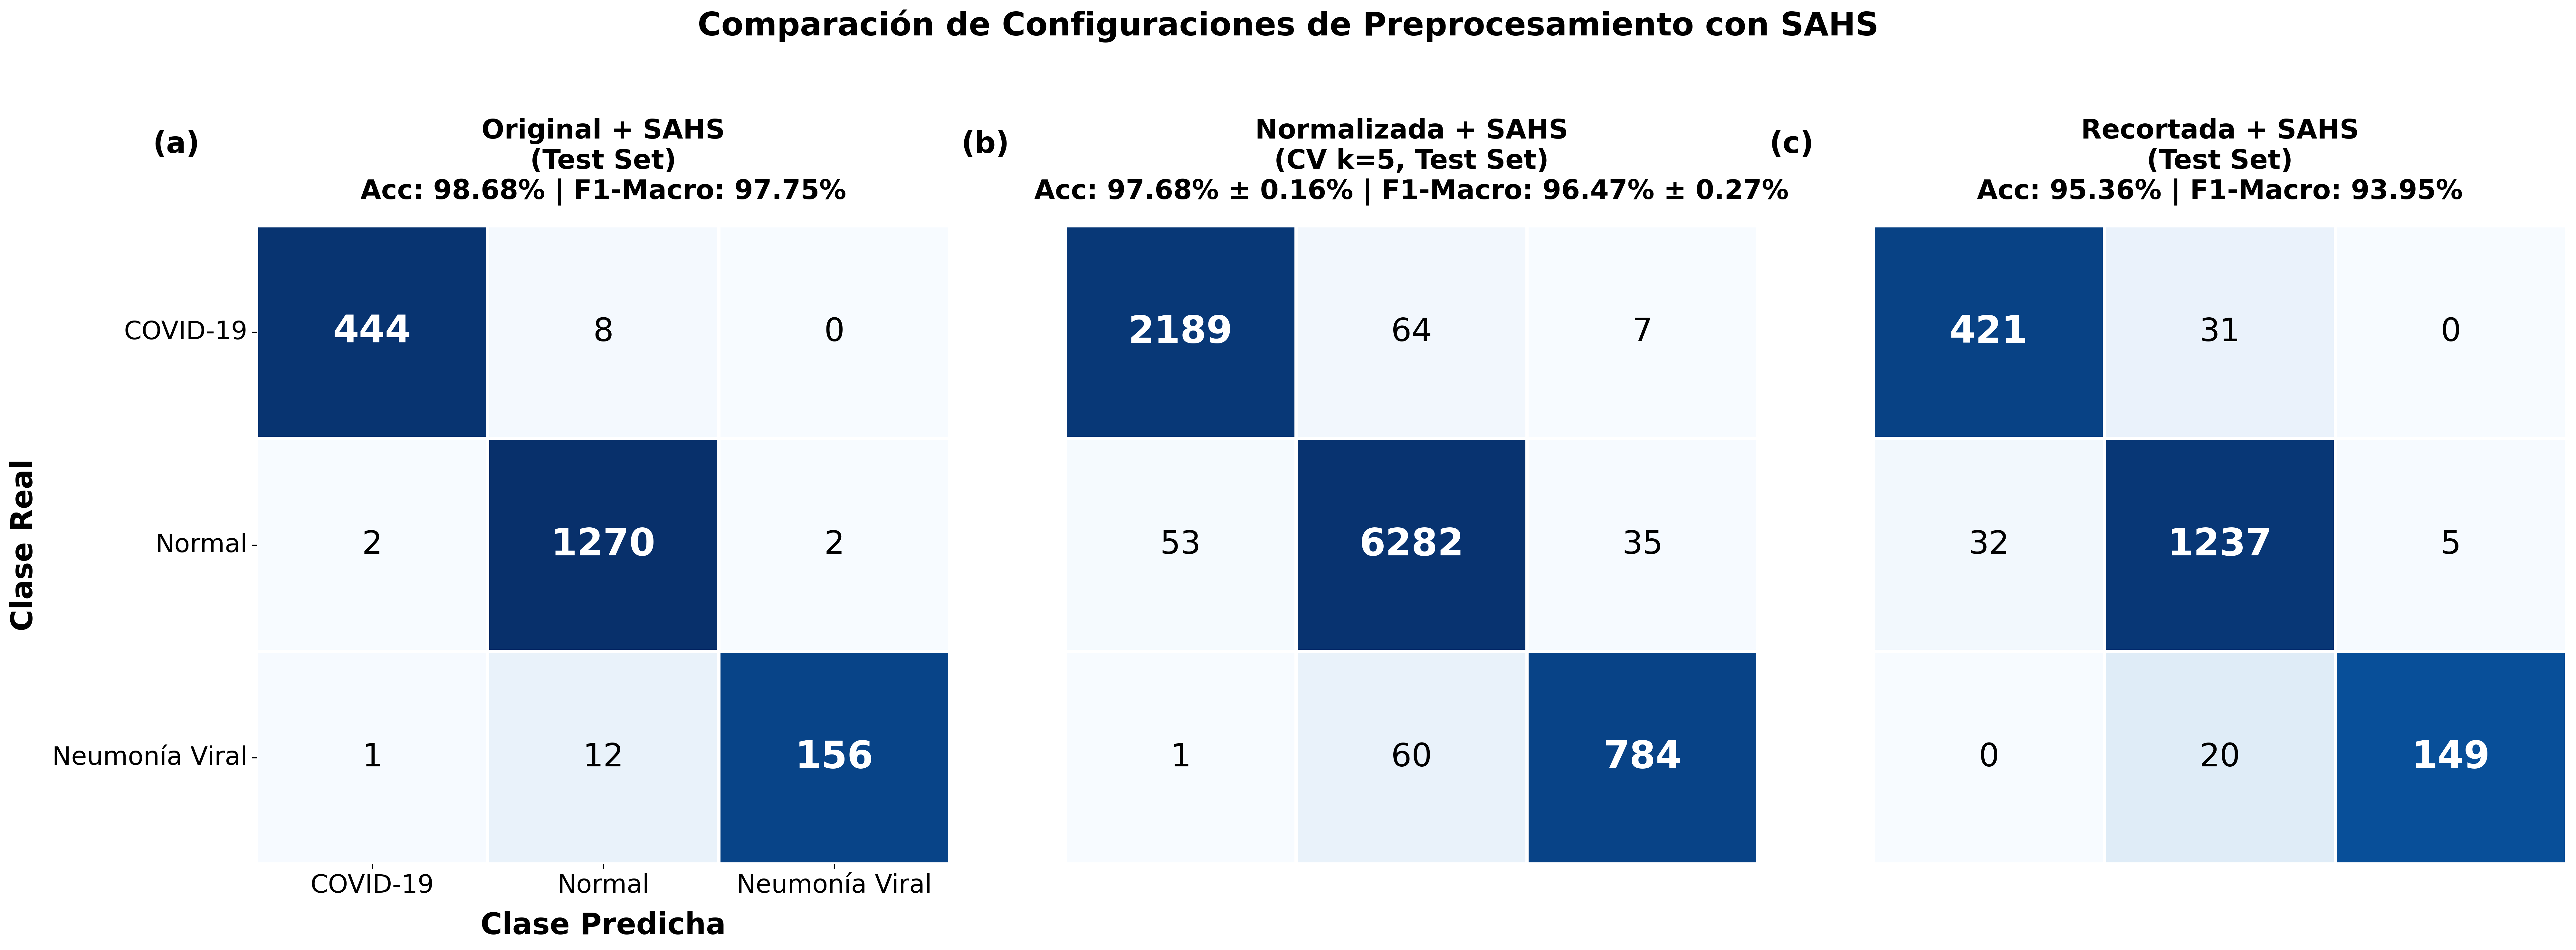
\includegraphics[width=0.99\textwidth]{Figures/F5.8_comparacion_cv.png}
    \caption{Comparación de matrices de confusión para las tres configuraciones de preprocesamiento. (a) Original + SAHS: 98.68\% de exactitud (test set). (b) Normalizado + SAHS (sistema propuesto): 98.60\% de exactitud (validación cruzada k=5, 13,258 muestras). (c) Recortado + SAHS: 95.36\% de exactitud (test set). La subfigura (b) usa validación cruzada para demostrar robustez estadística, alcanzando rendimiento equivalente a (a) con baja varianza ($\sigma = 0.26\%$). La caída de 3.32 puntos al recortar los bordes evidencia que las imágenes originales utilizan artefactos hospitalarios como características espurias.}
    \label{fig:comparacion_sahs_visual}
\end{figure}

\subsection{Resumen}
\label{subsec:resumen_clasificacion}

El sistema de clasificación basado en normalización geométrica alcanza los siguientes resultados mediante validación cruzada:

\begin{itemize}
    \item \textbf{Exactitud de 98.60\% $\pm$ 0.26\%} sobre 13,258 imágenes evaluadas mediante validación cruzada k=5.
    \item \textbf{F1-Score superior al 96.9\%} en las tres categorías diagnósticas.
    \item \textbf{F1-Score Macro de 98.00\% $\pm$ 0.36\%}, indicando rendimiento balanceado entre categorías.
    \item \textbf{Sensibilidad del 98.32\%} para detección de COVID-19.
    \item \textbf{Baja variabilidad entre folds} ($\sigma < 0.4\%$), confirmando estabilidad del modelo.
    \item Solo \textbf{186 errores} de clasificación en 13,258 imágenes (1.40\%).
\end{itemize}

El experimento comparativo de cuatro configuraciones (Original, Normalizado, ALP, Recortado) proporciona evidencia de que:

\begin{enumerate}
    \item \textbf{Las imágenes originales utilizan características espurias:} La caída consistente al eliminar bordes (3.32 puntos con recorte simple, 2.28 puntos con ALP inteligente) demuestra que las etiquetas hospitalarias contribuyen significativamente. Los resultados reportados por Picazo~\cite{picazo2023tesis} usando el mismo conjunto de datos validan nuestras observaciones.

    \item \textbf{La normalización geométrica aprende características genuinas:} El sistema propuesto (98.60\% con CV) mantiene alto rendimiento usando únicamente la región pulmonar normalizada con 15 puntos de referencia. La superioridad sobre el ALP (96.40\%, 4 puntos de referencia) se atribuye a mayor fidelidad anatómica y corrección geométrica explícita mediante GPA, Warping y SAHS. La equivalencia con imágenes originales (diferencia de 0.08\%) y la baja varianza ($\sigma = 0.26\%$) confirman que el modelo aprende características patológicas reales sin depender de atajos.

    \item \textbf{El recorte inteligente es superior al recorte simple:} El ALP (96.40\%) supera al recorte por porcentaje fijo (95.36\%) al adaptarse a la forma pulmonar individual. La variabilidad anatómica requiere métodos adaptativos, no recortes uniformes.

    \item \textbf{La exactitud de 98.68\% en imágenes originales está inflada:} Este valor no refleja capacidad para identificar patologías pulmonares, sino capacidad para explotar correlaciones espurias con artefactos hospitalarios en las esquinas.
\end{enumerate}

Adicionalmente, para validar la generalidad de la normalización geométrica, se evaluó un clasificador tradicional basado en reducción de dimensionalidad (PCA con 50 componentes, proyección discriminante de Fisher y KNN con K=21). Este clasificador alcanzó 80.44\% de exactitud sobre imágenes normalizadas geométricamente contra 77.06\% sobre imágenes originales, confirmando una mejora de +3.38 puntos porcentuales. Esta ganancia valida que el beneficio de la normalización no es específico de arquitecturas de aprendizaje profundo, sino que mejora la separabilidad entre clases de forma general.
